%************************************************
\chapter{Introduction}\label{ch:introduction}
%************************************************
\section{Survey}
%The thesis studies the computational methods used for non-coding ribonucleic acids (RNA) folding and inverse folding. This introductory chapter presents a general overview of the notions of nucleic acids, the biological motivation, the biochemical context and the implication of non-coding RNAs in the emerging field such as biotechnology and bioengineering. Those concepts will contribute to the understanding of the different topics considered throughout the course of this thesis. 

%Molecules in the cell participate in various biochemical reactions to maintain the proper structure and function of the cell. Some micro-molecules are small molecules of low weights; they are often referred to as monomers. Many micro-molecules can join together to form more complex molecules called macromolecules. There are four essential macromolecules in the cell: the nucleic acids, the lipids, the proteins and the carbohydrates. Nucleic acids carry the genetic blueprint and the instructions for the functioning of the cell. Lipids include fats, waxes, oils, hormones, and specific components of membranes and function as energy-storage molecules and chemical messengers. Proteins are one of the most abundant organic molecules in the living systems; they contribute to many functional activities: enzymatic catalyses, contractility, formation of selectively permeable membranes, reversible binding and transport, and immunological activities. Finally, carbohydrates are an essential part of our diet. They provide energy to the body; grains, fruits and vegetables are all considered natural sources of carbohydrates.

DNAs and RNAs are macromolecules in the nucleus of eukaryotic cells that allow storing information with the help of nucleotides. Nucleotides consist of a five-carbon sugar, a phosphate group, and a nucleobase. There are four nucleotides in the DNA, distinguished by their nucleobase: A for Adenine, T for Thymine, G for Guanine, and C for Cytosine. Similar to DNA, we also find four different nucleotides in RNA, distinguished by the nucleobase with only one exception; the Uracil (U), which replaces Thymine in DNA. Even though the basis blocks constituting the DNA were known for many years, in 1953, James Watson and Francis Crick \cite{watson1953molecular} succeeded in putting them together and suggested a reasonable DNA structure. 
Their work revealed for the first time that the structure of DNA molecules has helical chains, each coiled round the same axis where the chain consists of phosphate dieter groups. The two chains are held together by the purines and pyrimidine bases; they are joined together in pairs, a single base from the other chain bonded to a single base from the other chain. For the bounding to occur, one of the pairs must be Adenine and thymine or Guanine and Cytosine. A DNA molecule structure is depicted on the left side of the page. In contrast to DNA, RNAs are mostly single-stranded, and the complementary pairings formed in the structure are A-U, G-U and G-C.  
\graffito{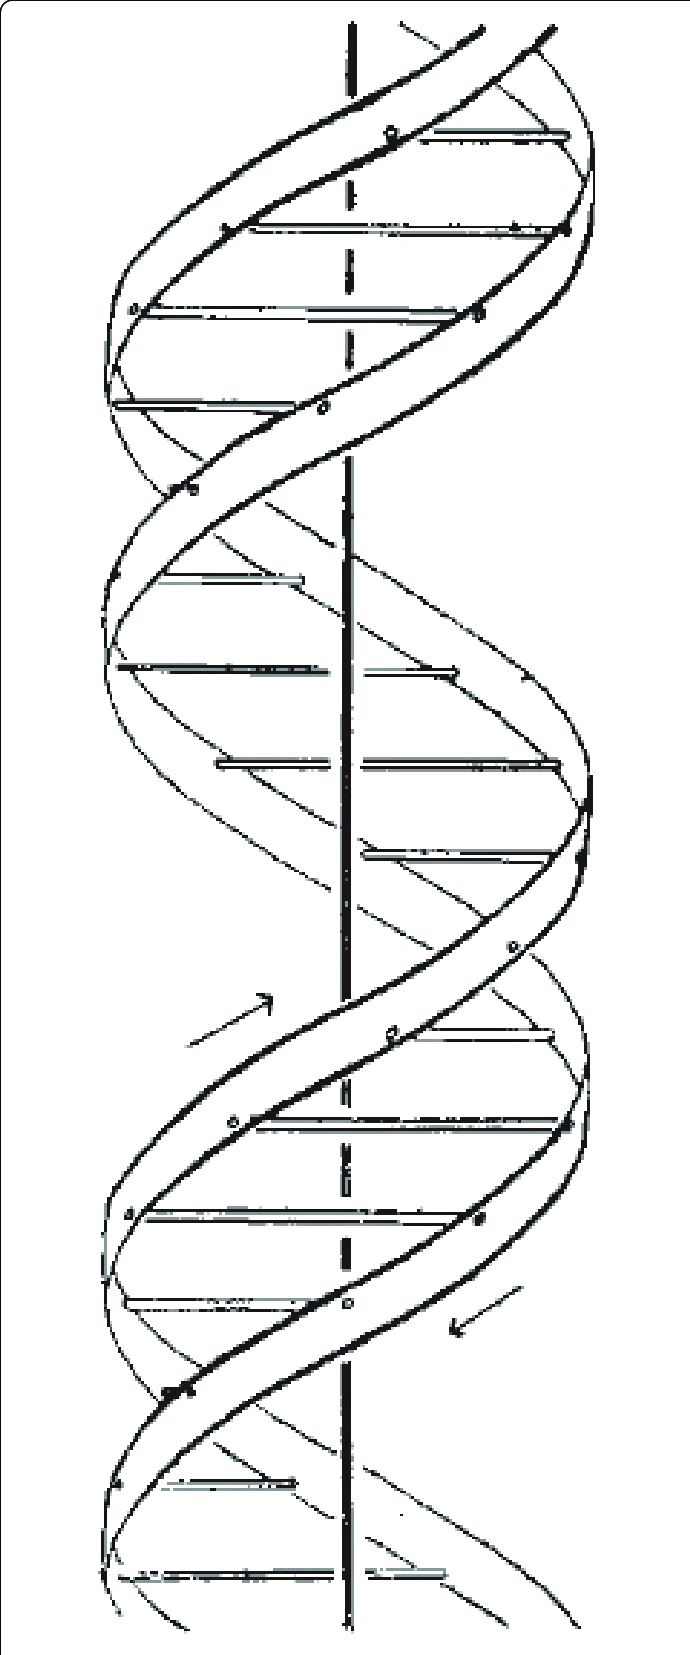
\includegraphics[width=1\linewidth]{../res/images/dna.png}
	Helical representation of DNA structures \cite{watson1953molecular}.}

Watson and Crick's elucidation of DNA structure has motivated many other scientists to investigate further the structural implications of molecules in functions such as replication and gave rise to modern molecular biology. Later in the same year, Crick formulated the central dogma of molecular biology that describes the flow of information between DNA, RNA, and proteins \cite{crick1970central}. He described the dogma in two steps: from DNA to mRNA through transcription and from mRNAs to proteins through translation. Since this central dogma was proposed, more works have been done to investigate each step. DNAs are transcribed into RNA molecules (messenger RNAs) that contain the same information as the template DNAs. Subsequently, these RNA messengers are translated into proteins according to the genetic code. But not all RNAs are translated into proteins; in other terms, not all RNAs are mRNAs. There are mainly two RNA groups: coding RNAs (cRNAs) translated into proteins and non-coding RNAs that are not translated into proteins. During the transcription and translation steps in the information flow, some vital functions are performed by non-coding RNAs such as ribosomal RNA (rRNAs) and transfer RNAs (tRNAs). The tertiary structure of a tRNA is shown on the right side of the page.
\graffito{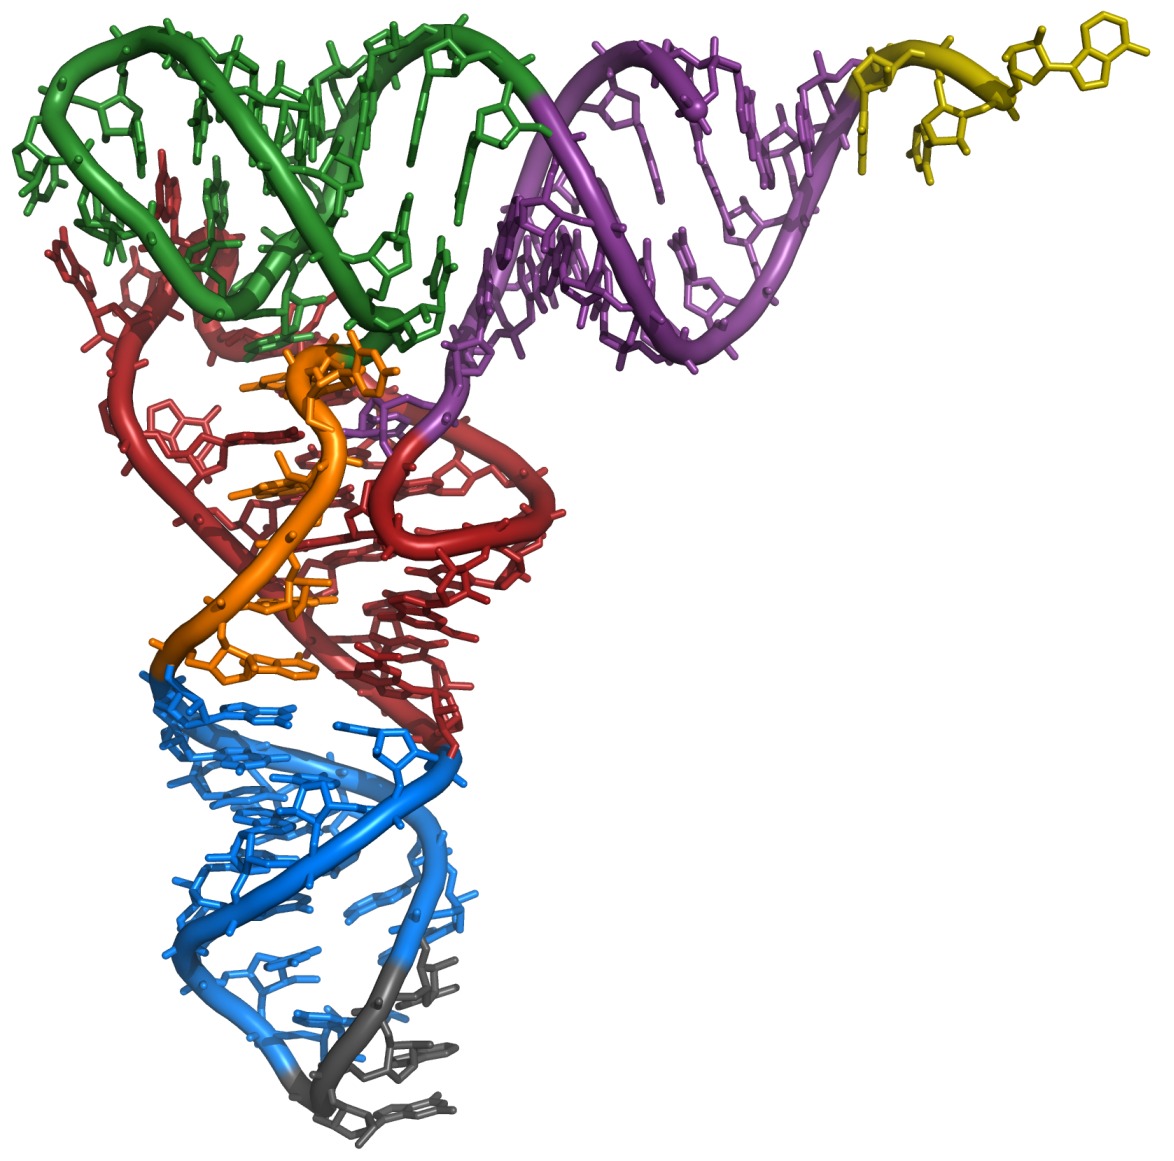
\includegraphics[width=1\linewidth]{../res/images/tertiary.png}
	The tertiary structure of tRNA. The CCA-tail is in yellow, the acceptor stem in purple, the variable loop in orange, D-arm in red, the anticodon arm in blue with anticodon in black, and T-arm in green (Taken from Wikipedia)}
The study of such RNAs revealed that rRNAs, rather than ribosomal proteins, catalyze the synthesis of proteins (i.e. the polymerization of amino acids), distinguish between correct and incorrect codon-anticodon pairs and prevent the premature hydrolysis of peptidyl-tRNAs \cite{moore2011roles, breaker2006rna}. Apart from being central to the protein machinery, ncRNAs regulate various biological functions in transcriptional interference, telomere maintenance, epigenetic changes, imprinting, post-transcriptional, translational control, structural organization, cell differentiation and development \cite{fatica2014long,santosh2015non}. 

The function of non-coding RNAs is largely determined by their high-dimensional structure \cite{cech2014noncoding}. For instance, we can analyze the catalytic function of ribozymes in terms of basic structural motifs, e.g. hammerhead or hairpin structures \cite{doherty2001ribozyme}. Other RNAs, like riboswitches, involve changes between alternative structures  \cite{vitreschak04_ribos}. Understanding the relation sequence and structure is a central challenge in molecular biology. In the last $20$ years, many different methods for determining the RNA structures of molecules have emerged: from experimental lab methods to computational approaches. For experimental lab methods, X-ray crystallography and the nuclear magnetic resonance (NMR)  are the most accurate approaches to offer structural information at a single base-pair resolution. Both experimental methods are often characterized by high experimental cost and low throughput. In addition to those limitations, RNA molecules are volatile and difficult to crystallize. Despite the development of more sophisticated techniques to infer the state of nucleotides in RNA molecules using enzymatic \cite{kertesz2010genome, underwood2010fragseq} or chemical probes \cite{tijerina2007dms, wilkinson2006selective} coupled with next-generation sequencing \cite{bevilacqua2016genome, tian2016rna}, most of them can only capture RNA structures \textit{in vitro} which mostly differ from the \textit{in vivo} structure conformations. Experimentally, only a tiny fraction of known ncRNAs has been determined \cite{rnacentral2017rnacentral}. Because measuring the structure of RNAs experimentally is very difficult and expensive, computational approaches play a central role in the analysis of natural RNAs \cite{seetin2012rna, fallmann2017recent}, and are an essential alternative to experimental approaches. RNAs fold into secondary structures before folding into higher-level (tertiary and quaternary) structures \cite{brion1997hierarchy,tinoco1999rna}. This separation of time scales justifies focusing on the secondary structure prediction; evidence suggests that the RNA's secondary structures largely determine the resulting high-level structures. 

This thesis focuses on computational methods addressing RNA molecules' folding and inverse folding at the secondary level. This introductory chapter presents a brief overview of the non-coding RNA concepts. The overview concepts contain biological and biochemical structure definitions of the non-coding RNAs. It also gives an overview of different techniques used to identify new ncRNA and some applications. It concludes by providing the bioinformatic definitions of RNA secondary structure that constitute the basis and understanding of computational methods and the results presented in this thesis.

%\section{DNAs, coding RNAs and non-coding RNAs}



\section{Characteristics and biological functions of  non-coding RNAs.} 
In the previous section, we introduced the central dogma of microbiology, which describes the flow of information in the living systems. Two important non-coding RNAs involved in the protein machinery have been highlighted. In this section, we provide some of the main characteristics of ncRNAs, and we emphasize how those characteristics often play an essential role in realizing their functions. 

What motivates the computational studies of ncRNAs is often the importance of the biological function they play. Consequently, the ncRNAs can be classified based on their biological functions. Although many recent transcriptomic and bioinformatic studies suggested thousands of ncRNAs with their functional importance, the total number of ncRNAs encoded in the human genome still remains unknown \cite{santosh2015non}. More recently, newly identified ncRNAs have not been validated by their function; it could be possible that most of them are non-functional. Some experiments \textit{in vitro} evolution have shown that RNA molecules can catalyze various chemical reactions relevant to biological processes such as RNA replication, nucleotide synthesis, thymidylate synthesis, lipid synthesis, and sugar metabolism \cite{robertson1990selection,ellington2009evolutionary}. 
Another characteristic of ncRNAs is their lengths formed post-transcriptionally. We often distinguish two main ncRNA classes of critical biological functions: the short non-coding RNAs (sncRNAs with length $<30nt$) and the long non-coding RNAs (lncRNAs with length $>200nt$). The length limit is often because of the practical considerations, including separating RNAs in standard experimental protocols. The length of non-coding RNAs is also taken into account in computational studies, and it will be used throughout our work to distinguish RNA sequences and structures in the different datasets considered.

The function of lncRNAs includes a role in higher-order chromosomal dynamics, telomere biology, and subcellular structural organization \cite{bergmann2014long,cusanelli2014telomeric}. Some lncRNAs play key regulatory and functional roles in the gene expression program of the cell. One of the vital functions is to act as ribozymes. Examples of naturally occurring ribozymes include group I and group II introns---RNase P and the hammerhead. The group, I and group II introns are usually $200-600$nt long, catalyzing RNA splicing. Many sncRNAs also contribute to the realization of similar biological functions. For example, small interfering RNAs contribute to gene regulation, transposon control and vital defence. MicroRNAs participate in the post-transcriptional gene regulation, microRNA-offset RNAs (moRNAs), PIWI-interacting RNAs (piRNAs) and promoter-associated RNAs (PARs) contribute to the gene regulation. More recently,  many discoveries revealed several non-coding RNAs implicated in cancer growth and MCL-1 expression regulation \cite{wang2021circpvt1, santosh2015non}. Those examples include ncRNAs from different classes, miRNAs, snoRNA and T-UCR, all associated with a specific disease \cite{santosh2015non,esteller2011non}. 

There are also other classes of ncRNAs such as Aptamers and riboswitches that have also been observed in nature. Aptamers are ncRNAs that can bind to other specified targets, whose nature is highly diverse. They range from small molecules to larger molecules. In some contexts, aptamers are termed riboswitches; for example, when their function is to sense the presence of an associated metabolite to cause a specific cis-reaction and/or cis-regulation of subordinated functional pathways \cite{winkler2003genetic}. 

In sum, lnc/snc-RNAs contribute to the realization of various biological functions, and they are mostly distinguishable based on their length. Their characteristics in terms of lengths are primarily due to the practical considerations in the standard experiments. But, their functions allow us to distinguish them better. In the next section, we provide some of the recent advancements in the techniques used to identify functional ncRNAs.

\section{Recent advancements in determining ncRNA functions}

Most of the previously mentioned functions of ncRNAs are identified using gene targeting techniques, a well-known technique used to investigate protein functions \cite{sauvageau2013multiple}. In addition, experimental approaches are used to define ncRNA functions. With the recent advancements in genome engineering, a method such as Clustered Regularly Interspaced Short Palindromic Repeats (CRISPR) has been employed to tag lncRNAs, allowing to capture specific RNA-protein complexes assembled \textit{in vivo}. 

The CRISPR \cite{barrangou2007crispr} was described by Barrangou and his collaborators in 2007 as a distinctive genome feature of most bacteria and archaea and thought to be involved in resistance to bacteriophages. It is an adaptive defence system against viruses and plasmid intrusions. When a successful defence takes place, the system updates information about the intruder's genetic material. This update will then allow the system's host to identify its enemy, making it robust and durable in the future. The information about the intruder's genetic material is stored in short repeating stretches of RNA, which can, in the case of a new intrusion, be incorporated into a carrier protein(CAS). The capacities of the  CRISPR/CAS9 of selectively destroying foreign DNA/RNA and editing the genome was identified by Li et al. \cite{li2016harnessing}, and it was turned into methods allowing to alter and edit single genes within genomes selectively. The same technology is also successfully applied to animal cell lines \cite{hwang2013efficient, jinek2013rna, wang2013one} and industrial plants \cite{svitashev2015targeted,li2015cas9}. 

Another method of SELEX (Systematic Evolution of Ligands by Exponential Enrichment) \cite{tuerk1990systematic} introduced by Tuerk in the early 1990s offers the possibility of enriching stretches of RNA that can bind towards a certain target. The method relies on mechanisms usually ascribed to the process of evolution, that is, variation, selection, and replication. A pool of RNAs that are entirely randomized at specific positions is subjected to selection for binding, in this case to GP43 on nitrocellulose filters. The selected RNAs are amplified as double-stranded DNA competent for subsequent in vitro transcription. This newly transcribed RNA is enriched for better binding sequences and is then subjected to selection to begin the next cycle. Multiple rounds of enrichment result in the exponential in the crease of the best binding ligands until they dominate the population of sequences. SELEX has given rise to numerous synthetic aptamers with different targets in its application. They have been subject to a further extension towards inclusion into regulative RNA entities.

More recently, increased types of ncRNAs have been detected and identified by the development of next-generation sequencing (NGS) \cite{wang2009rna}, which can be roughly divided into the process sections of sample preprocessing, library preparation, sequencing, and bioinformatics. 

The functions of many ncRNAs are dependent on their high-level structures, which often depend on a low-level ones such as secondary structures. Knowing the RNA structure of an ncRNA plays a vital role in probing its function. For example, it can help interpret experiments relating to the mechanism of RNA function \cite{flor1989conserved}. Or, it can help propose new experiments to probe function \cite{kim2007staufen1}. Therefore, understanding even the secondary structure alone can assist both of these examples. In the following section, we provide a biochemical definition of the secondary structure of ncRNAs and an overview of the different interactions involved during their formation. 


\section{Biochemistry of RNA molecules}\label{sec:rna_biochemical}

\graffito{
	\hspace*{-2cm}
	\scalebox{0.95}{
		
		\chemname[1cm]{\chemfig{
				-[,1.202,,,line width=3.5pt, shorten <=-.05pt, shorten >=-.05pt](-[:-90,,,,line width=1.5pt, shorten >=.5pt]OH)% 2
				>[:44.6,0.521](-[:90, 3.3]{\textcolor{blue}{Nucleobase}})
				-[:167]\chembelow[35pt]{O}{Ribose}
				-[:193,0.998]
				(
				-[:90](-[,0.1,,,draw=none]\chemabove[1ex]{}{\textcolor{gray}{5'}})
				-[::90,1.,,,red](-[::0,,,,red]\color{red}{P}(-[2,,,,red]\color{red}{O^{-}})(-[4,1.3,,,red]\color{red}{O^{-}})(=[6,,,,red]\chembelow{\color{red}{O}}{\textcolor{red}{Phosphate}}))
				)
				(
				<[:315.6,0.522](-[:-90,,,,line width=1.5pt, shorten >=.5pt]OH)(-[::-150,0.4,,,draw=none]\chembelow[1ex]{}{\textcolor{gray}{3'}})
				)
		}	}{Structure of an RNA nucleotide}
	}
	%	\vspace*{6cm}\\
	%	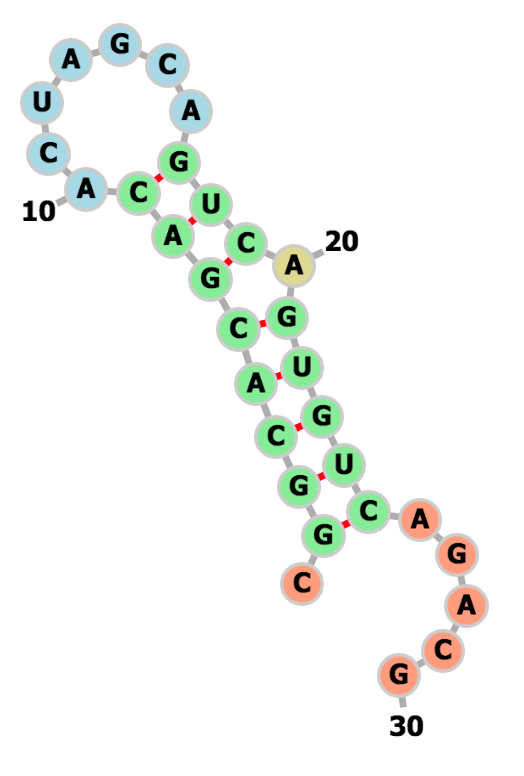
\includegraphics[width=1\linewidth]{../res/images/mfe.png}
	%	An example of secondary structure with a MFE of $8.5$kcal.$mol^{-1}$ (Produced using \texttt{RNAfold} from the \texttt{ViennaRNA} package)
}
So far in this work, we provided a biological motivation for studying non-coding RNA as an independent entity. The discovery of new ncRNAs functions has emerged through intensive experimental studies and with recent advanced techniques in next-generation sequencing. Several examples demonstrated the importance of the ncRNA structures in the probing process of new functions. The process in which RNA sequences are mapped to their corresponding structures is called RNA folding. In nature, this process is thought to be hierarchical \cite{brion1997hierarchy,tinoco1999rna}. Nucleotides form a chain given their sequence of bases (primary structure); RNAs fold into secondary structures, such as stem-loops and helices, before folding into higher-level (tertiary and quaternary) structures. Our work is restricted here to the secondary level of an RNA structure, i.e., the set of canonical pairs. This section provides a biochemical definition of different nucleotides and base-pair interactions involved in the secondary structure folding of RNA molecules. 

%\reversemarginpar

Chemically, each nucleotide in RNA molecules consists of a phosphate residue, a pentose sugar and a nucleobase. The typical chemical structure of a nucleotide is depicted on the right side of the page. Figure \ref{fig:nucleotide} illustrates the chemical structure of each of the four different nucleobases found in RNA (A, C, G and U). A nucleotide is a nucleoside which has a (mono, di, trip) phosphate residue bound to its 5'-carbon atom. By convention, the carbon atoms of the pentose sugar in nucleotides are numbered with \textit{primes}.

\begin{figure}[t!]
	\begin{minipage}[b]{.5\linewidth}
		\centering
		\subfloat[Adenosine 5'􏱈-monophosphate]{
			\label{fig:adenine}{
				\scalebox{0.9}{
					\chemfig{
						-[,1.202,,,line width=3.5pt](-[:-90,,,,line width=1.5pt]OH)% 2
						>[:44.6,0.521](-[:90] \color{blue}{N}*5(-[,,,,blue]*6(-[,,,,blue]\color{blue}{N}=[,,,,blue]-[,,,,blue]\color{blue}{N}=[,,,,blue](-[:90,,,,blue]\color{blue}{NH_2})-[,,,,blue]-[,,,,blue])=[,,,,blue]-[,,,,blue]\color{blue}{N}=[,,,,blue]-[,,,,blue]))
						-[:167]O
						-[:193,0.998]
						(
						-[:90](-[,0.1,,,draw=none]\chemabove[1ex]{}{\textcolor{gray}{5'}})
						-[::90]O(-[::0]P(-[2]O^{-})(-[4]O^{-})(=[6]O))
						)
						(
						<[:315.6,0.522](-[:-90,,,,line width=0.5pt]OH)(-[::-150,0.4,,,draw=none]\chembelow[1ex]{}{\textcolor{gray}{3'}})
						)
					}	
				}	
		}}\hfill
	\end{minipage}
	\begin{minipage}[b]{.5\linewidth}
		\centering		
		\subfloat[Uridine 5'-monophosphate]{
			\label{fig:uracil}{
				\scalebox{0.9}{\chemfig{
						-[,1.202,,,line width=3.5pt, shorten <=-.05pt, shorten >=-.05pt](-[:-90,,,,line width=1.5pt, shorten >=.5pt]OH)% 2
						>[:44.6,0.521](-[:90] \color{blue}{N}*6(-[,,,,blue](=[,,,,blue]\color{blue}{O})-[,,,,blue]\color{blue}{NH}-[,,,,blue](=[,,,,blue]\color{blue}{O})-[,,,,blue]=[,,,,blue]-[,,,,blue]))
						-[:167]O
						-[:193,0.998]
						(
						-[:90](-[,0.1,,,draw=none]\chemabove[1ex]{}{\textcolor{gray}{5'}})
						-[::90]O(-[::0]P(-[2]O^{-})(-[4]O^{-})(=[6]O))
						)
						(
						<[:315.6,0.522](-[:-90,,,,line width=1.5pt, shorten >=.5pt]OH)(-[::-150,0.4,,,draw=none]\chembelow[1ex]{}{\textcolor{gray}{3'}})
						)
				}}
		}}
	\end{minipage}
	
	\begin{minipage}[b]{.5\linewidth}
		\centering
		\subfloat[Cytidine 5'􏱈-monophosphate]{
			\label{fig:cytosine}{
				\scalebox{0.9}{	\chemfig{
						-[,1.202,,,line width=3.5pt, shorten <=-.05pt, shorten >=-.05pt](-[:-90,,,,line width=1.5pt, shorten >=.5pt]OH)% 2
						>[:44.6,0.521](-[:90]\color{blue}{N}*6(-[,,,,blue](=[,,,,blue]\color{blue}{O})-[,,,,blue]\color{blue}{N}=[,,,,blue](-[,,,,blue]\color{blue}{NH_2})-[,,,,blue]=[,,,,blue]-[,,,,blue]))
						-[:167]O
						-[:193,0.998]
						(
						-[:90](-[,0.1,,,draw=none]\chemabove[1ex]{}{\textcolor{gray}{5'}})
						-[::90]O(-[::0]P(-[2]O^{-})(-[4]O^{-})(=[6]O))
						)
						(
						<[:315.6,0.522](-[:-90,,,,line width=1.5pt, shorten >=.5pt]OH)(-[::-150,0.4,,,draw=none]\chembelow[1ex]{}{\textcolor{gray}{3'}})
						)
					}
				}
		}}
	\end{minipage}%
	\begin{minipage}[b]{.5\linewidth}
		\centering 
		\subfloat[Guanosine 5'􏱈-monophosphate]{
			\label{fig:guanine}{
				\scalebox{0.9}{	
					\chemfig{
						-[,1.202,,,line width=3.5pt, shorten <=-.05pt, shorten >=-.05pt](-[:-90,,,,line width=1.5pt, shorten >=.5pt]OH)% 2
						>[:44.6,0.521](-[:90] \color{blue}{N}*5(-[,,,,blue]*6(-[,,,,blue]\color{blue}{N}=[,,,,blue](-[,,,,blue]\color{blue}{NH_2})-[,,,,blue]\color{blue}{NH}=[,,,,blue](=[:90,,,,blue]\color{blue}{O})-[,,,,blue]-[,,,,blue])=[,,,,blue]-[,,,,blue]\color{blue}{N}=[,,,,blue]-[,,,,blue]))
						-[:167]O
						-[:193,0.998]
						(
						-[:90](-[,0.1,,,draw=none]\chemabove[1ex]{}{\textcolor{gray}{5'}})
						-[::90]O(-[::0]P(-[2]O^{-})(-[4]O^{-})(=[6]O))
						)
						(
						<[:315.6,0.522](-[:-90,,,,line width=1.5pt, shorten >=.5pt]OH)(-[::-150,0.4,,,draw=none]\chembelow[1ex]{}{\textcolor{gray}{3'}})
						)
					}
				}
				
		}}
	\end{minipage}%
	
	
	\caption{\textbf{RNA nucleotides.} Adenine and guanine belongs into the chemical class of purine molecules and the uracil and thymine in the class of pyrimidines}\label{fig:nucleotide}
\end{figure}

\graffito{
	%\vspace*{-5cm}\\
	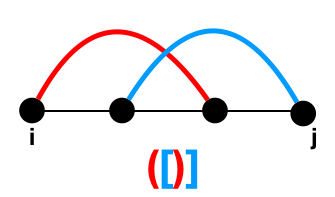
\includegraphics[width=1\linewidth]{../res/images/Hpk.png}
	Hairpin pseudoknot (H-type).
	
	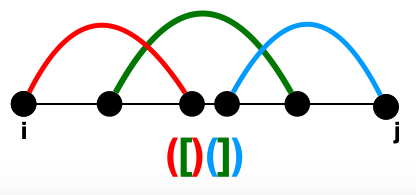
\includegraphics[width=1\linewidth]{../res/images/Kissingpk.png}
	Kissing hairpin pseudoknot (K-type). 
	
	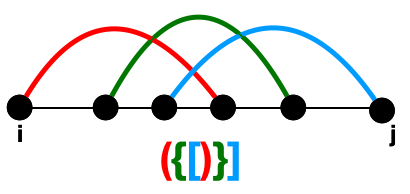
\includegraphics[width=1\linewidth]{../res/images/cHpk.png}
	Complex hairpin pseudoknot (CH-type).}

At the lowest level, RNA molecules are simply represented as a list of nucleobase characters. The 5'-3' phosphodiester bonds attach the different nucleotides composing the RNA molecule between ribose to form the primary structure of RNA. The chain direction is conventionally designed as 5' to 3' (i.e. from 5'-phosphate first sugar backbone to the 3'-hydroxyl last sugar in the sequence). 

In contrast to the RNA primary structure, the secondary structure consists of a list of nucleobase pairs, and the hydrogen bonds between the bases form base pairs. Different interactions are possible between the bases depending on the structure level considered. At the secondary level, we have the Watson-Crick (or canonical) pairs \cite{seeman1976rna, rosenberg1976rna} (A-U and G-C), the Wobble (or non-canonical) (G-U) pairs that occur with reduced frequency. Figure \ref{fig:basepairing} shows the chemical base pairs for the Watson-Crick and Wobble interactions. 


\begin{figure}
	%\hspace*{-4cm}
	\begin{minipage}[b]{1.0 \linewidth}
		\centering
		\subfloat[Adenine-Uracil Interaction]{
			\chemfig{
				R-[::42] N*5(
				%(-H)
				-(*6(
				-N=-N?[h1]
				=(-N([::60]-H)([::-60]-H?[h0]))-=
				))
				--N=-
				)
				*5(-[,,,,draw=none](*6(-[,,,,draw=none]-[,,,,draw=none]-[,,,,draw=none](-[,,,,draw=none]))))
				\phantom{A}-[,1.95,,,draw=none]
				-[::-60,2,,,draw=none]-[,2,,,draw=none]-[::120,,,,draw=none]
				N*6(%(-H)
				-=-(=O?[h0,,{dash pattern=on 1pt off 4pt}, {line width=1.5pt}, gray])-N(-H?[h1,,{dash pattern=on 1pt off 4pt}, {line width=1.5pt}, gray])-(=O?[h2,,{dash pattern=on 1pt off 4pt}, {line width=1.5pt}, gray])-)
				-[::180]R
			}
			
		}
	\end{minipage}
	\begin{minipage}[b]{1.0 \linewidth}
		\centering
		\subfloat[Guanine-Cytosine Interaction]{
			\chemfig{
				R-[::42]	N*5(
				%(-H)
				-(*6(
				-N=(-{NH_2})
				-N(-H?[h2])
				-(=O?[h1])-=
				))
				--N=-
				)
				*5(-[,,,,draw=none](*6(-[,,,,draw=none]-[,,,,draw=none]-[,,,,draw=none](-[,,,,draw=none]))))
				\phantom{A}-[,1.95,,,draw=none]
				-[::-60,2,,,draw=none]-[,2,,,draw=none]-[::120,,,,draw=none]
				*6()
				N*6(%(-H)
				-=-(-N([::60]-H?[h1,,{dash pattern=on 1pt off 4pt}, {line width=1.5pt}, gray])([::-60]-H))=N?[h2,,{dash pattern=on 1pt off 4pt}, {line width=1.5pt}, gray]-(=O?[h3,,{dash pattern=on 1pt off 4pt}, {line width=1.5pt}, gray])-)
				-[::180]R
			}
		}
		
	\end{minipage}
	%\vspace*{0.3cm}
	\begin{minipage}[b]{1.0\linewidth}
		\centering
		\subfloat[Guanine-Uracil Interaction]{
			\chemfig{
				R-[::42]	N*5(
				%(-H)
				-(*6(
				-N=(-{NH_2})
				-N(-H?[h2])
				-(=O?[h1])-=
				))
				--N=-
				)
				*5(-[,,,,draw=none](*6(-[,,,,draw=none]-[,,,,draw=none]-[,,,,draw=none]-[,,,,draw=none](-[,,,,draw=none]))))
				\phantom{A}-[,2.95,,,draw=none]
				-[::-60,2,,,draw=none]-[,2,,,draw=none]-[::120,,,,draw=none]
				N*6(%(-H)
				-=-(=O?[h0,,{dash pattern=on 1pt off 4pt}, {line width=1.5pt}, gray])-N(-H?[h1,,{dash pattern=on 1pt off 4pt}, {line width=1.5pt}, gray])-(=O?[h2,,{dash pattern=on 1pt off 4pt}, {line width=1.5pt}, gray])-)
				-[::180]R
			}
		}
	\end{minipage}
	
	\caption{\textbf{RNA base pair interactions.} (a) and (b) are commonly know as Watson-Crick base pairs. (c) is the wobble base pair. Hydrogen bonds are indicated as grey dashed lines. Substitution of bold hydrogen residues with ribose 5-phosphate yields the corresponding nucleotides found in RNA molecules.}\label{fig:basepairing}
\end{figure}


We also find crossing or pseudoknotted interactions in natural RNA that play vital roles in realising biological functions. Pseudoknots occur when two canonical or non-canonical interactions cross each other \cite{beyongWCpairs}. The three type of pseudoknot patterns often in RNA are depicted on the left side. Even though pseudoknots are often considered the beginning of the interaction between the secondary and tertiary levels of RNA structures, we consider them part of the secondary structure. Therefore, two main secondary structure definitions are considered in this work: a pseudoknot-free one in which only canonical interactions with no crossing pairs are allowed and a second one where canonical interactions with possible crossing pairs are permitted. The following section will provide formal definitions and the framework in which the folding of the secondary structure of ncRNAs can be computationally studied.

\section{Bioinformatic definitions.}

We provided in the previous sections the biological motivations and biochemical concepts that support the computation methods studied in the thesis. In order to computationally study and analyse RNA molecules, a more formal representation of RNAs and bioinformatic definitions are required. We provide in this section formal definitions and concepts that will support the result presented in this thesis.

\subsection{Structural definitions}
This thesis focuses on computational folding and inverse folding methods of the secondary structure of RNA molecules. The secondary structure, in most cases, is computed for a given RNA sequence. Along the thises, $\phi$ will represent an RNA sequence of a fixed length $L$ and $\mathcal{S}$ its corresponding structure. This subsection provides formal definitions of $\phi$, $\mathcal{S}$ and the structural properties of $\mathcal{S}$. We will assume the same definitions in the different tools reviewed in Chapters \ref{ch:folding}, \ref{ch:review_design}, and they support the different results presented in Chapters \ref{ch:rafft} and \ref{ch:arnaque}.

\paragraph{\textbf{Definition 1}} ( RNA sequence): More formally, $\phi$ consists of an ordered sequence of nucleotides that can be represented as:~ \begin{equation}
\phi\ =\ \left(\phi_1,...,\phi_L\right),
\end{equation}
where $\phi_i\in\left\{\text{A},\text{C},\text{G},\text{U}\right\}$ for $i\in \{1\dots L\}$.
\(\phi\)~is often known as the primary structure of RNA.

\paragraph{\textbf{Definition 2} } (RNA pseudoknot-free secondary structure): Given an RNA sequence $\phi \in \left\{\text{A},\text{C},\text{G},\text{U}\right\}^L$, let $\mathcal{P}=\big \{(i,j) \colon i<j \big \}$ be the list of possible pairing positions over the sequence $\phi$. A pseudoknot-free secondary structure $ \mathcal{S}\subset \mathcal{P} $ of such sequence $\phi$ is a list of base pairs  with the following constraints:
\begin{enumerate}
	\item A nucleotide (sequence position) can only belong to a single pair, i.e. $\forall (i,j), (k,l) \in \mathcal{S}$ with $i<k \colon i=k \Rightarrow j=l$.
	\item Paired bases must be separated by at least three
	unpaired nucleotides. i.e. \(\forall (i,j) \in \mathcal{S} \Rightarrow \) \(j-i\geq3\).
	\item There are no pseudoknots, i.e. $ \nexists \left(i,j\right), \left(k,l\right) \in \mathcal{S}$
	~with~\(i<k<j<l\),
	\item The base pairs consist exclusively of Watson–Crick ($C–G$ and $A–U$) pairs and Wobble ($G–U$) pairs. i.e. $\forall \left(i,j\right) \in \mathcal{S}\Rightarrow \phi_i\phi_j \in \left\{\text{GC},\text{CG},\text{AU},\text{UA},\text{GU},\text{UG}\right\}$,
\end{enumerate}

%Throughout this thesis, this definition is considered when benchmarking the 
\paragraph{\textbf{Definition 3} } (Secondary structure representation): A graphical way of representing an RNA secondary structure. There are several representations of $\mathcal{S}$. 
\begin{itemize}
	\item Dot-bracket (or string) representation: In this representation, the secondary structure $\mathcal{S}$  is compactly stored in a string $\sigma$ consisting of dots and matching brackets. i.e.  $\sigma$ is a string of length $L$ over the alphabet $\Delta_{\sigma}= \big\{ (,),[,],\{,\},<,>,.\big\}$ where, at each unpaired positions we have a dot '.' at the corresponding string position, and $\forall (i,j) \in \mathcal{S}$, we have an opening bracket at position $\sigma_i$ and a closing bracket at position $\sigma_j$. We denote $\sigma$ the string representation of the structure $\mathcal{S}$. Figure \ref{fig:representation}D shows an example of a string representation.
	\item Planar representation: it is the common way of representing an RNA secondary structure in which $\mathcal{S}$ is presented as a graph with each vertex representing a nucleotide  and an edge connecting consecutive nucleotides and base pairs (See Figure \ref{fig:representation}B). 
	\item Circular (or circle ) representation: similar to planar representation, $\mathcal{S}$  is a graph but drawn in the plane in such a way that all vertices are arranged on a circle, and the edges representing base pairs lie inside the circle. In a pseudoknot-free secondary structure circular representation, the edges do not intersect (See Figure \ref{fig:representation}A).  
	\item Linear representation: In this representation, $\mathcal{S}$  is a graph in which the nucleotides are arranged consecutively in a line and the edges representing base pairs form semi-circle that do not intersect for pseudoknot-free structure (See Figure \ref{fig:representation}C).
	\item Mountain representation: it is mainly used for representing large structures. $\mathcal{S}$  is presented in a two-dimensional graph, in which the $x$-coordinate is the position $i$ of the nucleotide in the sequence $\phi$ and the $y$-coordinate the number $m(i)$ of base pairs that enclose nucleotide $i$.
	\item Tree representation: $\mathcal{S}$  is drawn as a tree in which internal nodes are the base pairing positions, and the leaves are the unpaired positions. The dot-bracket representation is also often considered as a tree represented by a string of parenthesis (base pairs) and dots for the leaf nodes (unpaired nucleotides). 
	\item Shapiro representation: it allows representing the different elements composing $\mathcal{S}$  by single matching brackets, and the components are labelled with H(Hairpin), B(Bulge), I (interior loop), M (multi-loop) and S (stacking loop) \cite{shapiro1990comparing}.
\end{itemize}
Figure \ref{fig:representation} shows some examples of RNA secondary structure representation. For graphical illustrating examples in the thesis, we will mostly use the planar representation, and for computational methods will use the dot-bracket representation for simplicity.  
\begin{figure}
	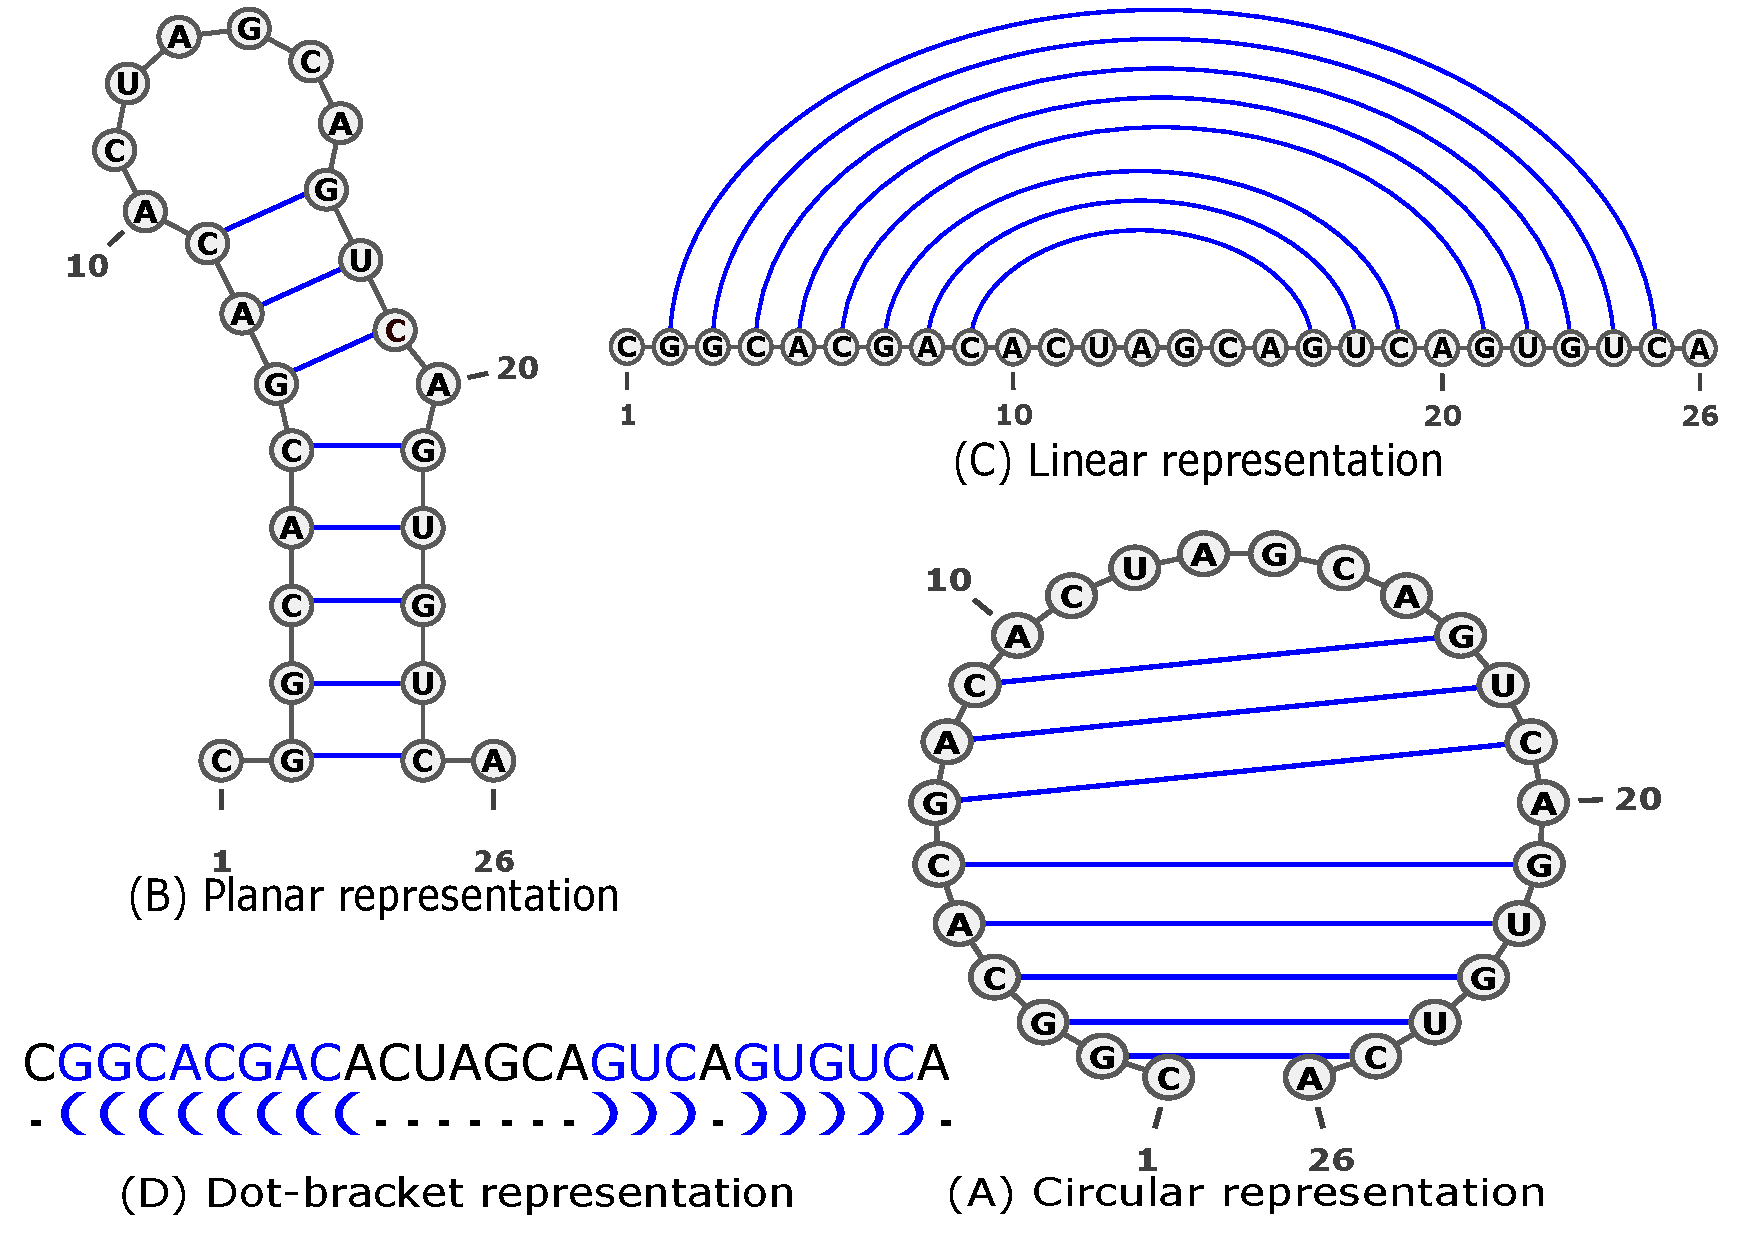
\includegraphics[width=1. \linewidth]{../res/images/arnaque/rep.pdf}
	\caption{\textbf{RNA secondary structure representation}}\label{fig:representation}
\end{figure}


\paragraph{\textbf{Definition 4} }(Secondary structure loop):  
\graffito{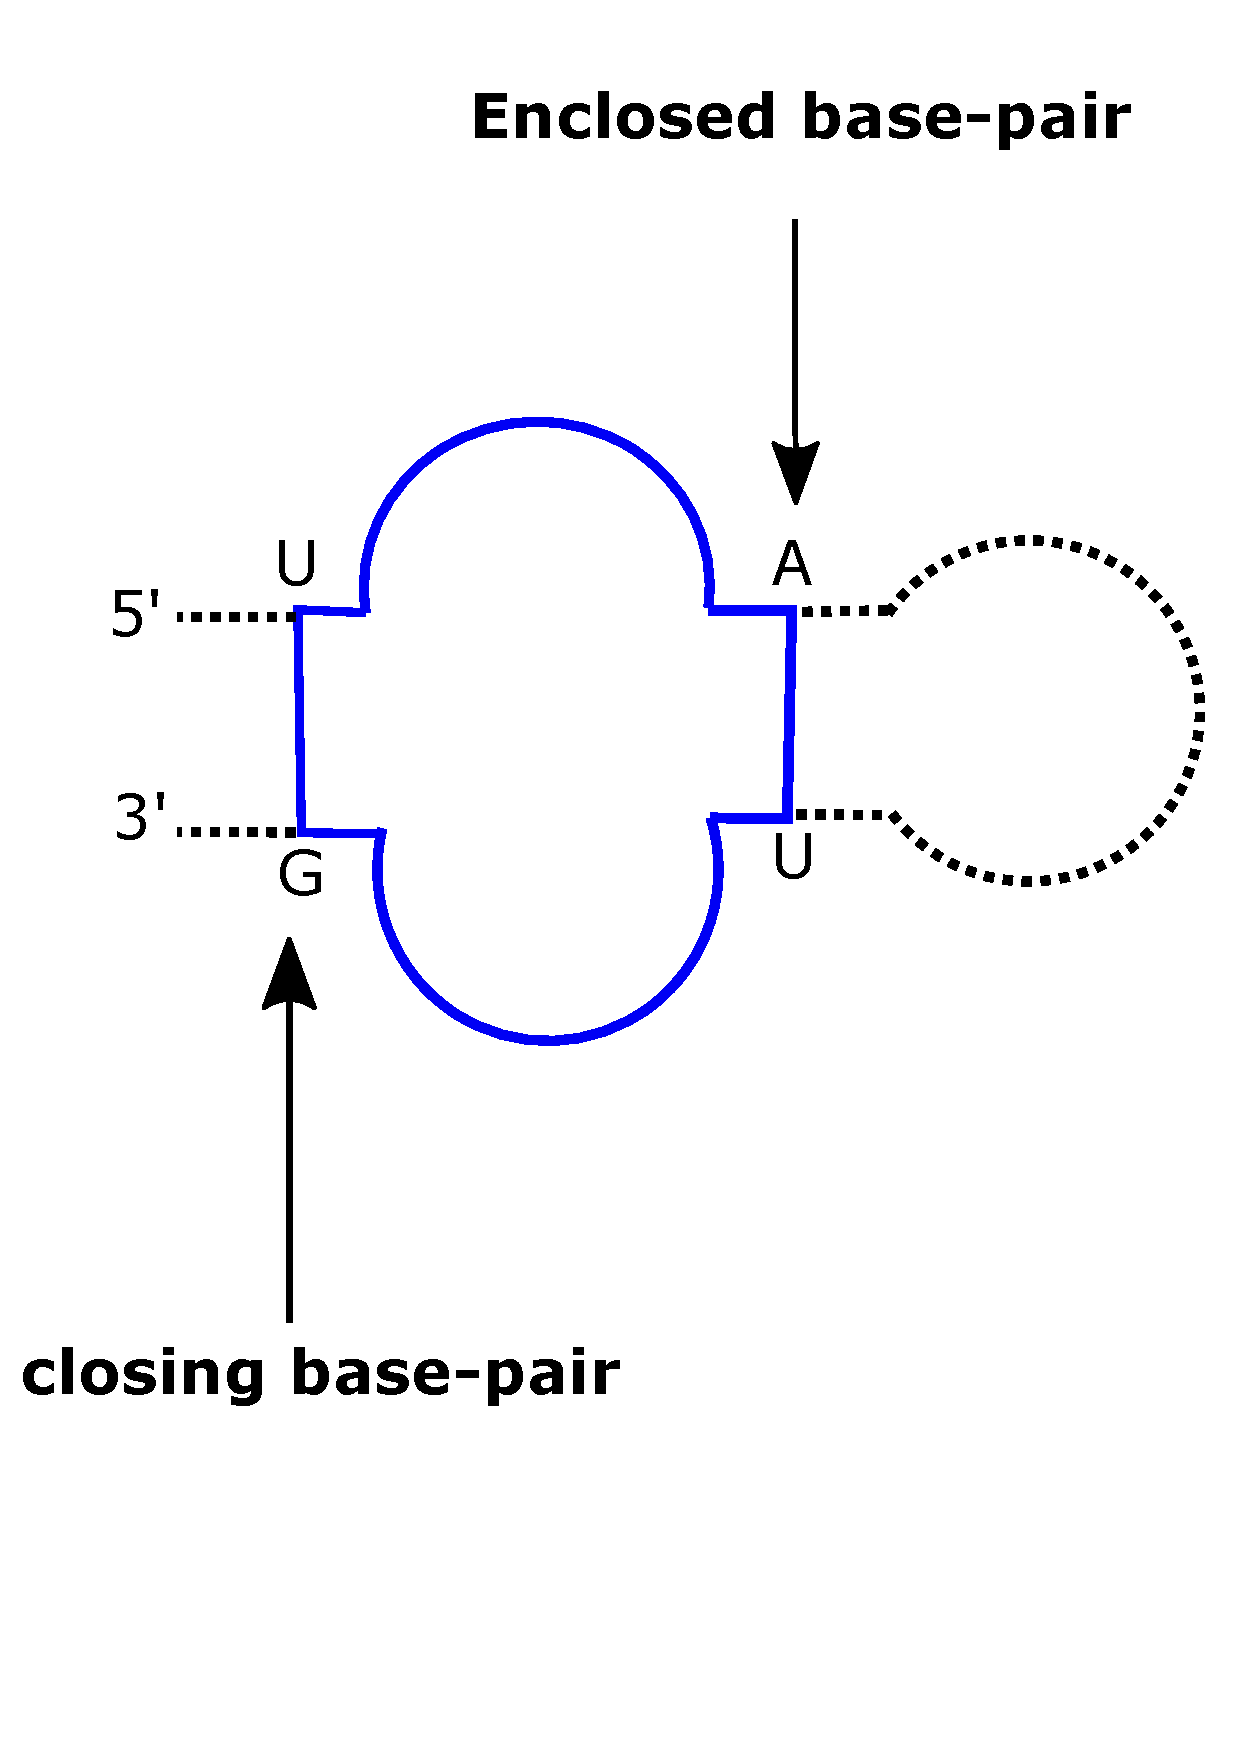
\includegraphics[width=1\linewidth]{../res/images/interior.pdf}
	An example of closing and enclosed base pairs of an interior loop.
}
There exists a unique decomposition of $\mathcal{S}$ into a set of $n$ loops $\mathbb{L}_{\phi, \mathcal{S}}$, where loops are the faces of its planar drawing. Each loop $\mathcal{L} \in \mathbb{L}_{\phi, \mathcal{S}}$ is characterised by its length $l$ (the number of unpaired nucleotides in the loop) and its degree $d$ (the number of base pairs delimiting the loop, including the closing loop pair). 

By definition, $\forall  \mathcal{L} \in \mathbb{L}_{\phi, \mathcal{S}} \Rightarrow \mathcal{L}  = \mathcal{L}_p \cup \mathcal{L}_u$ where $\mathcal{L}_p$ and $\mathcal{L}_u$ denote respectively the set of loop base pairs and the unpaired positions. $\mathcal{L}_p$ contains only one closing loop and the rest are enclosed base pairs. We say $(i,j) \in \mathcal{L}_p$ is a closing pair if and only if $\forall \mathcal{L}_p \ni (i',j') \neq (i,j) \colon i<i'<j'<j$.


\begin{enumerate}
	\item Interior loop: a loop with degree $d=2$ i.e $|\mathcal{L}_p|=2$ and $\mathcal{L}_u \subset \{1,2,\dots L\}\cup \emptyset$.
	\item Stacking pair: an interior loop of length $l=0$ i.e. $|\mathcal{L}_p|=2$ and $\mathcal{L}_u = \emptyset$.
	\item Hairpin Loop: Any loop of degree $d=1$ and length $l \geq 3$.  i.e $|\mathcal{L}_p|=1$ and  $\mathcal{L}_u \neq \emptyset$.
	\item Bulge loop: a special case of interior loop in which there are unpaired bases only on one side. i.e  $\mathcal{L}_p=\{(i_1,j_1), (i_2, j_2)\}$ with $i_1 \neq i_2, j_1\neq j_2$ one of the following assumption holds: 
		\begin{itemize}
			\item If $\exists i'\in \mathcal{L}_u \colon i_1<i'<j_2 \Rightarrow \nexists k'\in \mathcal{L}_u \colon i_2<k'<j_2$ 
			\item If $\exists k'\in \mathcal{L}_u \colon i_2<k'<j_2 \Rightarrow \nexists i'\in \mathcal{L}_u \colon i_1<i'<j_1$ 
		\end{itemize}
	\item Multi-loop: Any loop with degree $d>2$ i.e.  $|\mathcal{L}i_p| \geq 3$  and $\mathcal{L}_u \neq \emptyset$.
	\item Exterior loop: a loop in which all the positions are not interior of any pair i.e. $\mathcal{L}_p=\emptyset$ and $\mathcal{L}_u \neq \emptyset$.
\end{enumerate}

\begin{figure}[H]
	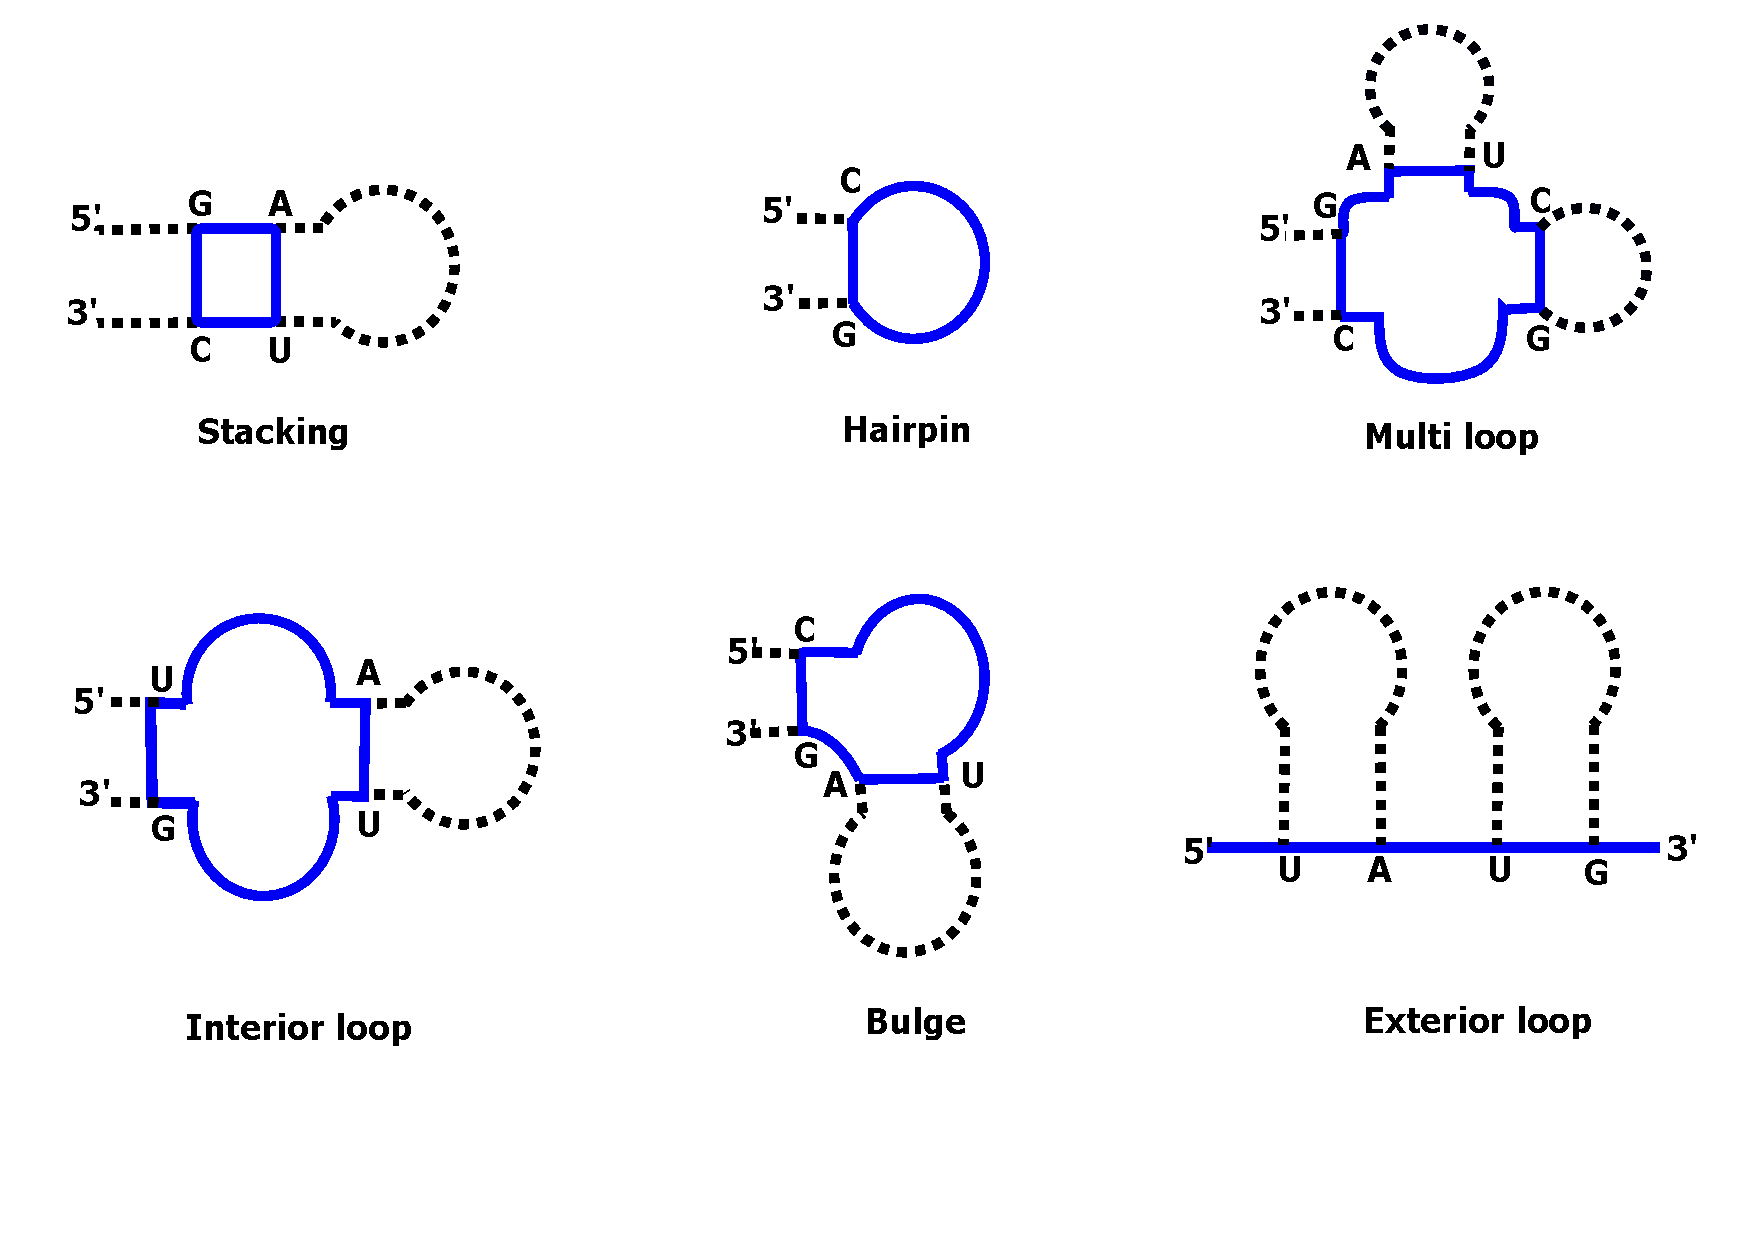
\includegraphics[width=1.0 \linewidth]{../res/images/loops.pdf}
	\caption{\textbf{RNA secondary structure loop decomposition}. Each loop is highlighted in blue.}\label{fig:loops}
\end{figure}

\paragraph{\textbf{Definition 5}} (Free Energy of an RNA secondary structure): Given the loop set $\mathbb{L}_{\phi, \mathcal{S}}$, the free energy \(\Delta G\) of $\mathcal{S}$ defines its thermodynamic stability. \(\Delta G\) is the free energy difference with respect to the completely unfolded state \cite{tinoco_estimation_1971}. \(\Delta G (\mathcal{S}, \phi)\) is computed using the additivity principle \cite{dill97_addit_princ_bioch}, by summing up the energies of its constituent loops.
\begin{equation}
	 \Delta G(\mathcal{S}, \phi) = \sum_{\mathcal{L}\in \mathbb{L}_{\mathcal{S}, \phi}}{ \Delta G(\mathcal{L}) }
\end{equation}
Many models allow for computing the free energies of those constituent loops, but the dominant is the nearest-neighbor loop energy model \cite{turner09_nndb}. This model associates tabulated free energy values to loop types and nucleotide compositions; the Turner2004 \cite{mathews2004incorporating} is one of the most widely used parameter sets. 

The free energy of each given loop $\mathcal{L}$ is expressed as
\begin{equation}\label{eq:gibbs}
\Delta G (\mathcal{L}) = \Delta H - T \Delta S \leq 0
\end{equation}
where $\Delta H$ is the (pressure- and volume-dependent) enthalpy change, $T$ the absolute temperature and $\Delta S$ the entropy change. 
The dominant stabilizing effect is attributed to consecutive base pairs (The stacking loops), whereas long unpaired regions enclosed between base pairs have destabilizing effects \cite{fresco_molecular_1960, hofacker_rna_2006}. As a simplified example, the destabilizing free energy contribution $\Delta G(\mathcal{L}_m)$ of a multiloop $\mathcal{L}_m$  as seen in \ref{fig:loops}C is modelled as:
\begin{equation}\label{eq:multi}
\Delta G(\mathcal{L}_m) = \Delta G_\mathrm{init} + b \Delta G_\mathrm{branch} + u \Delta G_\mathrm{unpaired}
\end{equation}
where $b$ is the number of all surrounding base pairs and $u$ the number of base pairs \parencite{dirks_partition_2003}.
The structure decomposition and the tabulated energy parameter sets allow an efficient dynamic programming algorithm to determine a sequence's minimum free energy (MFE) structure in the entire structure space. A literature review of tools using such techniques is given in Chapter \ref{ch:folding} of the thesis.
\subsection{Thermodynamic definitions}
A common way to computationally address RNA folding is to consider RNA folding as a dynamic system of structures ( the states of the system). Given enough time, a sequence $\phi$ will form every possible structure $\Sigma_{\phi}$. For each structure $\mathcal{S} \in \Sigma_{\phi}$,  there is a probability of observing it at a given time. This subsection defines RNA folding thermodynamic properties such as structural ensemble, partition function, Boltzmann probability of a structure $\mathcal{S}$, and the others that derive from them, the base-pair probability and the most probable secondary structure. 

The folding tools such as \texttt{RNAfold}, \texttt{LinearFold} used in this thesis use the same thermodynamic definitions. However, some computational folding methods do not rely on a thermodynamic model. For example, Chapter \ref{ch:folding} presents a literature review of such tools. 

\paragraph{\textbf{Definition 6}}  (Structure Ensemble):  For a given RNA sequence $\phi$,  the set of all pseudoknot-free secondary structures with their corresponding energies is called the structure ensemble $\Sigma_{\phi}$ of $\phi$ or Boltzmann ensemble.  We write: 

$$
\Sigma_{\phi} = \{ \mathcal{S} | \mathcal{S} \text{ is a secondary structure of $\phi$}\}
$$

According to the nearest neighbor energy model, all possible secondary structures of a given RNA sequence do not have the same energy. Since each structure has a unique decomposition, each structure has its own energy but different structures can have the same energy.

\paragraph{\textbf{Definition 7}} (Partition function of RNA): Given the free energy change $\Delta G(\mathcal{S})$ of a structure $\mathcal{S}$, the partition function $Z(\Sigma_{\phi})$ is defined on the Boltzmann ensemble (or structure ensemble) of all possible structures of a given sequence $\phi$ and we write: 

\begin{equation}
	Z(\Sigma_{\phi}) = \sum_{\mathcal{S} \in \Sigma_{\phi} }{\exp(-\beta \Delta G(\mathcal{S}, \phi))}
\end{equation}

Where, $\beta = (RT)^{-1}$ with $R$ the ideal gas constant, and $T$ the temperature.

\paragraph{\textbf{Definition 8}} (Secondary structure probability):
How probable is an RNA secondary structure $\mathcal{S} \in \Sigma_{\phi}$ for the sequence $\phi$? Given the free energy change $\Delta G(\mathcal{S})$ of a structure $\mathcal{S}$, the boltzmann distribution describes the structure's probability at constant temperature $T$ among all other possible structure of the same sequence $\phi$.
The probability $p(\mathcal{S}| \phi)$ depends on the free energy $\Delta G(\mathcal{S})$, the lower the more probable. We write: 

\begin{equation}
	p(\mathcal{S}| \phi)= \frac{\exp(-\beta \Delta G(\mathcal{S}, \phi))}{Z}
\end{equation}

where, $Z$ is the partition function and $\beta = (RT)^{-1}$ the thermal constant. 


\paragraph{\textbf{Definition 9}} (MFE secondary structure): 
To predict biologically relevant structures, most computational methods search for structures that minimize the free energy. For a given sequence $\phi$, let~\(\Sigma_{\phi}\) be the secondary structure ensemble of~\(\phi\). The minimum free energy structure $\mathcal{S}_{MFE}$ is the structure with the lowest probability $p(\mathcal{S}|\phi)$ i.e. the  most stable conformation in the thermodynamic equilibrium. We write:

\begin{equation}
\mathcal{S}^{MFE}(\phi) = \arg \min_{\mathcal{S} \in \Sigma_{\phi}} \Delta G(\mathcal{S}, \phi) 
\end{equation}

\paragraph{\textbf{Definition 10}}(Base pair probability): Let $\phi=(\phi_i)_{1\leq i \leq L} $ be an RNA sequence. The base pair probability matrix $\mathbf{P}(\phi)$ quantifies the equilibrium structural features of the ensemble $\Sigma_{\phi}$, with entries $P_{i,j}(\phi) \in [ 0,1]$ defines as follows: 

\begin{equation}
	P_{i,j}(\phi) = \sum_{\mathcal{S} \in \Sigma_{\phi}}{p(\mathcal{S}|\phi)S_{i,j}(\mathcal{S})}
\end{equation} 

$P_{i,j}(\phi)$ corresponds to the probability that base pair $i.j$ forms at the equilibrium. 
\(\mathbf{S}(\mathcal{S})\) is the structure matrix with entries \(S_{i,j} \in  \{ 0, 1\}\). If the structure \(\mathcal{S}\) contains pair~ $(i ,j)$, then \(S_{i,j}(\mathcal{S}) = 1\)~otherwise \(S_{i,j}(\mathcal{S}) = 0\).

\subsection{Structural distance definitions }
The validation of the results obtained in this thesis is purely empirical. We achieved this goal by comparing the predicted and expected structures for the folding tools. We use the PPV and the sensitivity's statistical properties for the benchmark results presented in Chapter \ref{ch:rafft}. For the inverse folding tools, we compare the MFE structure of the designed sequence to the target structure. For that end, a rigorous definition of a measure of similarities between two structures is needed. This subsection defines the different similarity measurements used throughout this work. In addition, it defines the objective functions used in our inverse folding presented in Chapter \ref{ch:arnaque} (Definitions 16 and 17). 
\paragraph{\textbf{Definition 11}}  The positive predictive value (PPV):  it measures the fraction of correct base pairs in the predicted structure and it is defined as follows: 

\begin{equation}
	PPV = \frac{TP}{TP + FP}
\end{equation}

where TP and FP stand respectively for the number of correctly predicted base pairs (true positives), and the number of wrongly predicted base pairs (false positives). 

\paragraph{\textbf{Definition 14}} (Sensitivity): it measures the fraction of
base pairs in the accepted structure that are predicted.
\begin{equation}
\text{Sensitivity} = \frac{TP}{TP+FN}
\end{equation}
where FN stands for the number of base pairs not detected (false
negatives).

\paragraph{\textbf{Definition 12}} (Base pair distance):  Let $\sigma_1$ and $\sigma_2$ be two secondary structures in their string representation.  The base pair distance between $\sigma_1$ and $\sigma_2$ is defined as follows: 
\begin{equation}
d_{bp}(\sigma_1, \sigma_2 )= \sum_{i,j} A_{i,j}[\sigma_1] + A_{i,j}[\sigma_2] + 2\times A_{i,j}[\sigma_1] A_{i,j}[\sigma_2],
\end{equation}
where, 
$$
A_{i,j}[\sigma] =
\begin{cases}
1 & \text{if $(i,j)$ is a base pair in $\sigma$ } \\
0 & \text{otherwise}
\end{cases}
$$

\paragraph{\textbf{Definition 13}} (Hamming Distance):  Let $\sigma_1$ and $\sigma_2$ be two secondary structures in their string representation. We define the hamming distance between $\sigma_1$ and $\sigma_2$, $d_h(\sigma_1, \sigma_2)$, to be the number of position where $\sigma_1$ and $\sigma_2$ differ.  

\begin{equation}
	\label{eq:hamming}
	d_h(\sigma_1, \sigma_2) = \sum_{i=1}^{L}{S(\sigma_1^i, \sigma_2^i)}
\end{equation}
where, 
$$
S(\sigma_1^i, \sigma_2^j) =
\begin{cases}
1 & \text{if $\sigma_1^i \neq \sigma_2^j)$ } \\
0 & \text{otherwise}
\end{cases}
$$
\paragraph{\textbf{Definition 14}} (Ensemble defect (ED)) \citep{zadeh2011nucleic}: Given an RNA sequence $\phi$ of length $L$, the ensemble defect $\mathcal{D}_E$ is the expected base pair distance between a target structure $\mathcal{S}^*$  and a random structure generated with respect to the Boltzmann probability distribution. It is defined as follows: 

\begin{equation}
\label{ed}
\begin{split}
\mathcal{D}_E(\phi, \mathcal{S}^*) 
&= \sum_{\mathcal{S} \in \Sigma_{\phi}}{p(\mathcal{S}|\phi)d_{bp}(\mathcal{S},\mathcal{S}^*)}\\
&= L - \sum_{1<i,j<L} P_{i,j}(\phi)S_{i,j}(\mathcal{S}^*)
\end{split}
\end{equation}

where~\(P_{i,j}\)~is the base pair probability matrix entrances, $d_{bp} ((\mathcal{S},\mathcal{S}^*))$ is the base pair distance between two structures, and \(\mathbf{S}(\mathcal{S})\) is the structure matrix with entries \(S_{i,j} \in  \{ 0, 1\}\). If the structure \(\mathcal{S}\) contains pair~ $(i ,j)$, then \(S_{i,j}(\mathcal{S}) = 1\)~otherwise \(S_{i,j}(\mathcal{S}) = 0\).

\paragraph{\textbf{Definition 15} } Normalized Energy Distance (NED): the difference between
the energy of a given sequence~\(\phi\)~evaluated to fold into a target structure $\mathcal{S}^*$ and the minimum free energy of the sequence in its structural ensemble~\(\Sigma_{\phi}\).~ The value is normalized over all the sequences in a given population $P$.  


\begin{equation}
\label{ned}
\mathcal{N}_E (\phi, \mathcal{S}^*) = [1-\Delta \hat{E}(\mathcal{S}^*,\phi)]^q \text{   } \forall q>1
\end{equation}
where,
\begin{equation}
\Delta \hat{E}(\mathcal{S}^*, \phi) = \frac{\Delta E(\mathcal{S}^*, \phi) }{\sum_{s \in P}{\Delta E(\mathcal{S}^*, s)}}
\end{equation}
and,
\begin{equation}
\Delta E(\mathcal{S}^*,\phi) = \Delta G(\mathcal{S}^*, \phi) - \arg \min_{\mathcal{S} \in \Sigma_{\phi\\
}} \Delta G(\mathcal{S}, \phi)
\end{equation}


\subsection{RNA folding map properties}
This work considers RNA molecule folding and inverse folding optimisation problems. In both cases, It is fundamental to define the fitness landscape notion. This subsection provides the formal definitions of the fitness landscape and examples related to the folding and inverse problem. Some properties such as neutrality, mutation mode or move operator are also provided. The size of the RNA structural ensemble has been analytically computed through tools developed by Stein and Waterman \cite{stein1979some}, and it yields an upper bound of~\(S_L\approx1.48\times L^{-\frac{3}{2}}1.85^L\) structure vis-a-vis~\(4^L\) sequences. Compared to the total number of sequences, the number of structures is much smaller, which means there is a high possibility that many sequences fold into the same MFE secondary structure. In case that happens, we call the set of those sequences a neutral set. The fraction of such sequences defines the neutrality of a fitness landscape.

\paragraph{\textbf{Definition 16}} (Fitness landscape) :  A fitness landscape $\mathfrak{L}$ results from the combination of three elements: a set of configurations $\mathcal{V}$, a cost or fitness function $f$, and a \textit{move} operator $\psi$ that induces a topology on the set of configurations. We write: 

\begin{equation}
	\mathfrak{L} = (\mathcal{G}_f, f, \psi)
\end{equation}

where $\mathcal{G}_f$  is the the landscape underlying the hypergraph whose vertices are the elements from $\mathcal{V}$ labelled with values given by $f$, and whose edges are specified by the move operator $\psi$.

The fitness function $f$ assigns to each configuration $v\in \mathcal{V}$ a real value taken from an interval $ \mathbb{I} \subset \mathbb{R}$ as follows: 

$$
f: \mathcal{V} \rightarrow \mathbb{I}
$$

An example of fitness function in the case of inverse folding is defined in Chapter \ref{ch:arnaque} (Section \ref{sec:objective_function}), which uses the hamming distance $d_h$ and $\mathcal{V}=\left\{ \text{A}, \text{C}, \text{G}, \text{U} \right\}^L$. But in this case, the fitness defined in the structural space $\Sigma_{\phi}$. i.e. we have an intermediate folding function $\Delta G (\mathcal{S}, \phi)$, mapping any sequence $\phi \in \mathcal{V}$ to an MFE secondary structure. 

The move (or mutation) operator $\psi$ defines the relationship between the configuration from  $\mathcal{V}$ in the following way: 
$$
\psi \colon \mathcal{V} \rightarrow \mathcal{V} 
$$
\paragraph{\textbf{Definition 17}} (Mutation mode): 
Let $\phi, \phi' \in \mathcal{V} = \left\{ \text{A}, \text{C}, \text{G}, \text{U} \right\}^L$, be  two RNA sequences. $\phi'$ is said to be an $n$-point mutation of $\phi$ if it differs from $\phi$ at $n$ nucleotides; i.e. $d_h(\phi, \phi')=n$ where $d_h(.,.)$ is the hamming distance on $\left\{ \text{A}, \text{C}, \text{G}, \text{U} \right\}^L$. 

A mutation mode is a random variable $U$ taking values in $\{1,\dots,L\}$. $P(U=n)$ is defined as the probability that, exactly $n$ nucleotides, selected uniformly at random undergo point mutation during a mutation event. $U$ can generally be any probability distribution.


\paragraph{\textbf{Definition 18}} (Neutral set of RNA sequences): For a give fitness landscape 
$\mathfrak{L} = (\mathcal{G}_f, f, \psi)$, with $\mathcal{V} = \left\{ \text{A}, \text{C}, \text{G}, \text{U} \right\}^L$, two RNA sequence $\phi_1$ and $\phi_2$  are set to be neutral $\iff f(\phi_1) = f(\phi_2)$. We call a set $\Gamma \subset \mathcal{V}$ of all such RNA sequences a neutral set.  In the case of inverse folding, $\phi_1$ and $\phi_2$ are neutral if they share the same MFE secondary structure. In contrast, $\phi_1$ and $\phi_2$ have the same free energy in the folding problem context. 

\paragraph{\textbf{Definition 19}} (Neutral Network): Let $\mathcal{G} (\mathcal{V}, E)$ be a connected graph in which vertices are all in the neutral sequence set $\Gamma$ (i.e. $\mathcal{V} \subset \Gamma$).  $\mathcal{G}$ is said to be a neutral network $\iff \forall e(v_i, v_j) \in E $,  $v_i,v_j$ differ by a single nucleotide (i.e. $d_h(v_i, v_j)=1$).
%\reversemarginpar
%\graffito{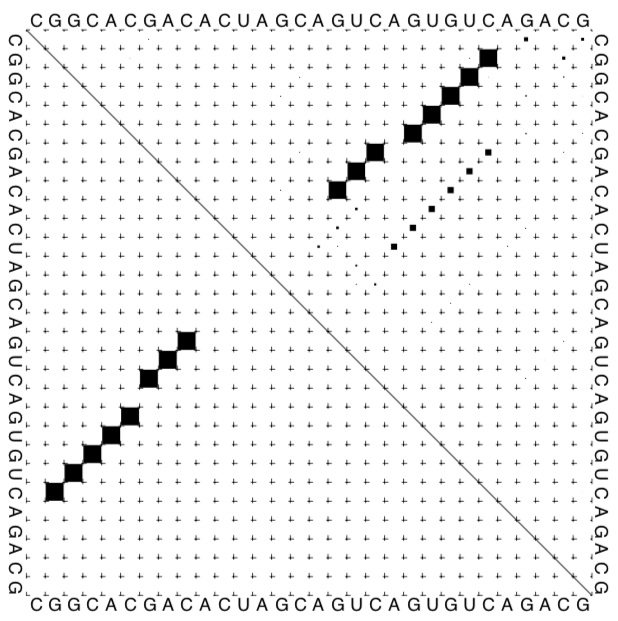
\includegraphics[width=1\linewidth]{../res/images/prob.png}
%	An example of the base pair matrix probabilities.}


%\paragraph{\textbf{Definition 18}} (Local minima): 

%\paragraph{\textbf{Definition 19}} (Global minima): 

%\paragraph{\textbf{Definition 20}} (Lévy Flights): 

%\paragraph{\textbf{Definition 21} }(Local search): 

\section{Conclusion and outline of the thesis}

This introductory chapter presents nucleic acids in general and, in particular, a description of RNA and its chemical, biological, and algorithmic definitions. Those concepts with biological motivations constitute the basis of the thesis. 

We organize the next part of the thesis into five chapters. The two first chapters are grouped into a first result part which only concerns the RNA folding. The second part discusses inverse folding, and similarly to the first part, it contains two chapters. The last chapter discusses the presented results and concludes by providing some limitations and possible future research directions. 

In this first result part, Chapter \ref{ch:folding} provides a brief literature review on the existing computational methods for RNA folding. The review focuses on thermodynamic and machine learning methods such as \texttt{RNAfold}, \texttt{LinearFold} and \texttt{Mxfold}. The methods presented in Chapter \ref{ch:folding} have some limitations, such as the computational time, and in some cases, the predicted thermodynamic structure does not match the native one. Chapter \ref{ch:rafft} presents our proposed folding tool called \texttt{RAFFT}, which aims at overcoming those limitations. \texttt{RAFFT} implements a novel heuristic to predict RNA secondary structure formation pathways that has two components: (i) a folding algorithm and (ii) a kinetic ansatz. This heuristic is inspired by the kinetic partitioning mechanism, by which molecules follow alternative folding pathways to their native structure, some much faster than others. \texttt{RAFFT} starts by generating an ensemble of concurrent folding pathways ending in multiple metastable structures, which contrasts with traditional thermodynamic approaches that find single structures with minimal free energies. When analyzing $50$ predicted folds per sequence, we found near-native predictions for RNAs of length $\leq 200$ nucleotides, matching the performance of current deep-learning-based structure prediction methods. \texttt{RAFFT} also acts as a folding kinetic ansatz, which we tested on two RNAs: the coronavirus frameshifting stimulation element (CFSE) and a classic bi-stable sequence. For the CFSE, an ensemble of $68$ distinct structures computed by \texttt{RAFFT} allowed us to produce complete folding kinetic trajectories. In contrast, known methods require evaluating millions of sub-optimal structures to achieve this result. For the second application, only $46$ distinct structures were required to reproduce the kinetics, whereas known methods required a sample of $20,000$ structures. 

Similar to the first part of the result, the second part contains two chapters. Chapter \ref{ch:review_design} will briefly introduce the RNA design problem. It distinguishes the positive from the negative RNA design problem and reviews the current state of art computational tools, especially those implementing evolutionary techniques. The existing tools present challenges when benchmarked on recent datasets such as \texttt{Eterna100}. Another limitation is that most existing tools do not consider the pseudoknot patterns in their designing process. In Chapter \ref{ch:arnaque}, we proposed an improved evolutionary algorithm inspired by the Lévy flights. Like a Lévy flight, our tool, \texttt{aRNAque}, implements a Lévy mutation scheme that allows simultaneous search at all scales over the landscape. New mutations often produce nearby sequences (one-point mutations) but occasionally generate mutant sequences far away in genotype space (macro-mutations). In \texttt{aRNAque}, the number of point mutations distribution at every step is taken to follow a Zipf distribution. The Lévy mutation scheme increases the diversity of designed RNA sequences and reduces the average number of evaluations of the evolutionary algorithm compared to the local search. The overall performance showed improved empirical results compared to existing tools through intensive benchmarks on both pseudoknot (the \texttt{PseudoBase++} dataset) and pseudoknot-free ( the \texttt{Eterna100} dataset) datasets. 

Finally, Chapter \ref{ch:conclusion} presents a general conclusion, a discussion on the results obtained and some promising perspectives. It emphasizes the understanding of the Lévy mutation in the context of RNA design and the connection of our results to evolutionary dynamics. 
